

\section{Introduction}

This project compares two deep learning architectures on an image classification task: a Convolutional Neural Network (CNN) and a Vision Transformer (ViT). Both models are built from scratch in TensorFlow/Keras and trained to classify rice grain images into five varieties . The goal is to evaluate how each architecture performs under identical conditions, without any pretraining or transfer learning.

The core question is whether the CNN's spatial inductive bias gives it a meaningful advantage over the ViT's global self-attention when both are trained from scratch on a domain-specific dataset.

\section{Dataset and Preprocessing}

The dataset is the Rice Image Dataset, containing roughly 75,000 JPEG images across five classes: Arborio, Basmati, Ipsala, Jasmine, and Karacadag . All images are resized to 224x224 pixels and scaled to the float range.

The data is split into 70\% training, 15\% validation, and 15\% test using stratified sampling to keep class proportions equal across splits . A fixed random seed (42) is used throughout for reproducibility. Training images receive augmentation in the form of random horizontal flips, rotations up to 10\%, and zoom up to 10\% . Validation and test images are not augmented. Class weights are computed from the training split and passed to the optimizer to handle any class imbalance. Data loading uses tf.data with prefetching and parallel mapping for efficient GPU throughput .

\section{Model Architectures}

\begin{minipage}{0.48\linewidth}
\subsection{CNN}

The CNN is a sequential model built from three convolutional blocks followed by a fully connected classification head. The general pattern in each block is to apply a convolution to extract spatial features, activate with ReLU, and then reduce spatial dimensions with max pooling. As the network deepens, the number of filters increases, allowing later layers to detect more complex and abstract patterns.

\textbf{Block 1} applies a \texttt{Conv2D} layer with 32 filters of size $3 \times 3$ and ReLU activation, followed by \texttt{MaxPooling2D}, which halves the spatial resolution from $224 \times 224$ to $112 \times 112$.

\textbf{Block 2} repeats the same structure with 64 filters, reducing the spatial dimensions further to $56 \times 56$. The increased filter count allows the layer to capture more feature channels simultaneously.

\textbf{Block 3} uses 128 filters and again halves the spatial size to $28 \times 28$. After the pooling step, a \texttt{Dropout} layer with rate 0.3 is applied to reduce overfitting by randomly deactivating neurons during training.

The \textbf{classification head} flattens the resulting feature map into a one-dimensional vector, passes it through a \texttt{Dense} layer with 128 units and ReLU activation, applies \texttt{Dropout} with rate 0.4, and finally outputs class probabilities through a \texttt{Dense} layer with 5 units and softmax activation.
  \end{minipage}
  \hfill
  \begin{minipage}{0.48\linewidth}
   \begin{figure}[H]
    \centering
    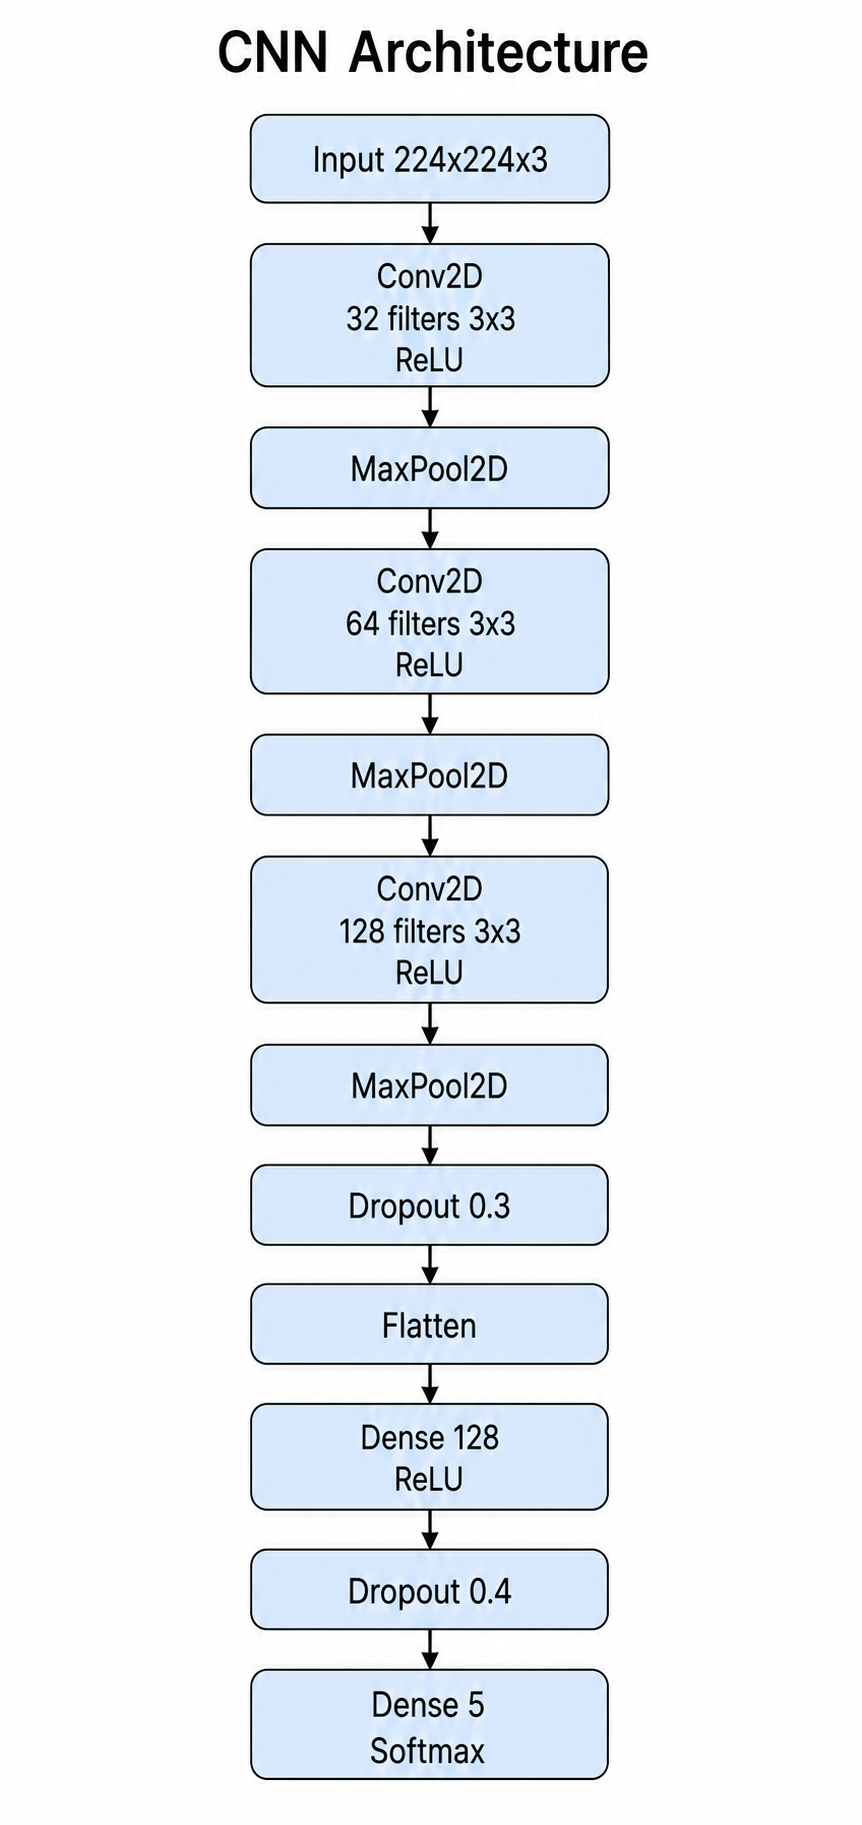
\includegraphics[width=\linewidth]{figures/cnn2.png}
  \caption{CNN model overview.}
  \label{fig:cnn}
\end{figure}
  \end{minipage}

\subsection{Vision Transformer}
The ViT is implemented from scratch in Keras. Rather than processing the image
pixel by pixel or region by region as a CNN does, the ViT first converts the
image into a sequence of patch embeddings and then processes that sequence with a stack of Transformer encoder blocks.

\begin{minipage}{0.48\linewidth}

\textbf{Patch embedding.} The $224 \times 224$ input image is divided into non-overlapping patches of size $16 \times 16$, producing $(224 / 16)^2 = 196$ patches. This is implemented with a single \texttt{Conv2D} layer using kernel size 16 and stride 16, which simultaneously extracts each patch and projects it into a 64-dimensional embedding vector. The output is reshaped to a sequence of 196 vectors, each of dimension 64.

\textbf{Positional encoding.} Unlike CNNs, self-attention has no built-in notion of position. To compensate, a learned \texttt{Embedding} layer maps each of the 196 position indices to a 64-dimensional vector, which is added element-wise to the patch embeddings. This allows the model to learn which positions matter for a given task.

\textbf{Transformer encoder.} The sequence passes through six stacked encoder blocks. Each block consists of two sub-layers, both with residual connections. The first sub-layer applies \texttt{LayerNormalization} followed by \texttt{MultiHeadAttention} with 4 heads and key dimension 64. Attention allows every patch to attend to every other patch in the sequence, so the model can capture global relationships across the image regardless of spatial distance. The second sub-layer applies another \texttt{LayerNormalization} followed by a two-layer MLP with hidden dimensions 128 and 64 and GELU activation. Dropout with rate 0.1 is applied inside both the attention layer and the MLP.

  \end{minipage}
  \hfill
\begin{minipage}{0.48\linewidth}
    \centering
    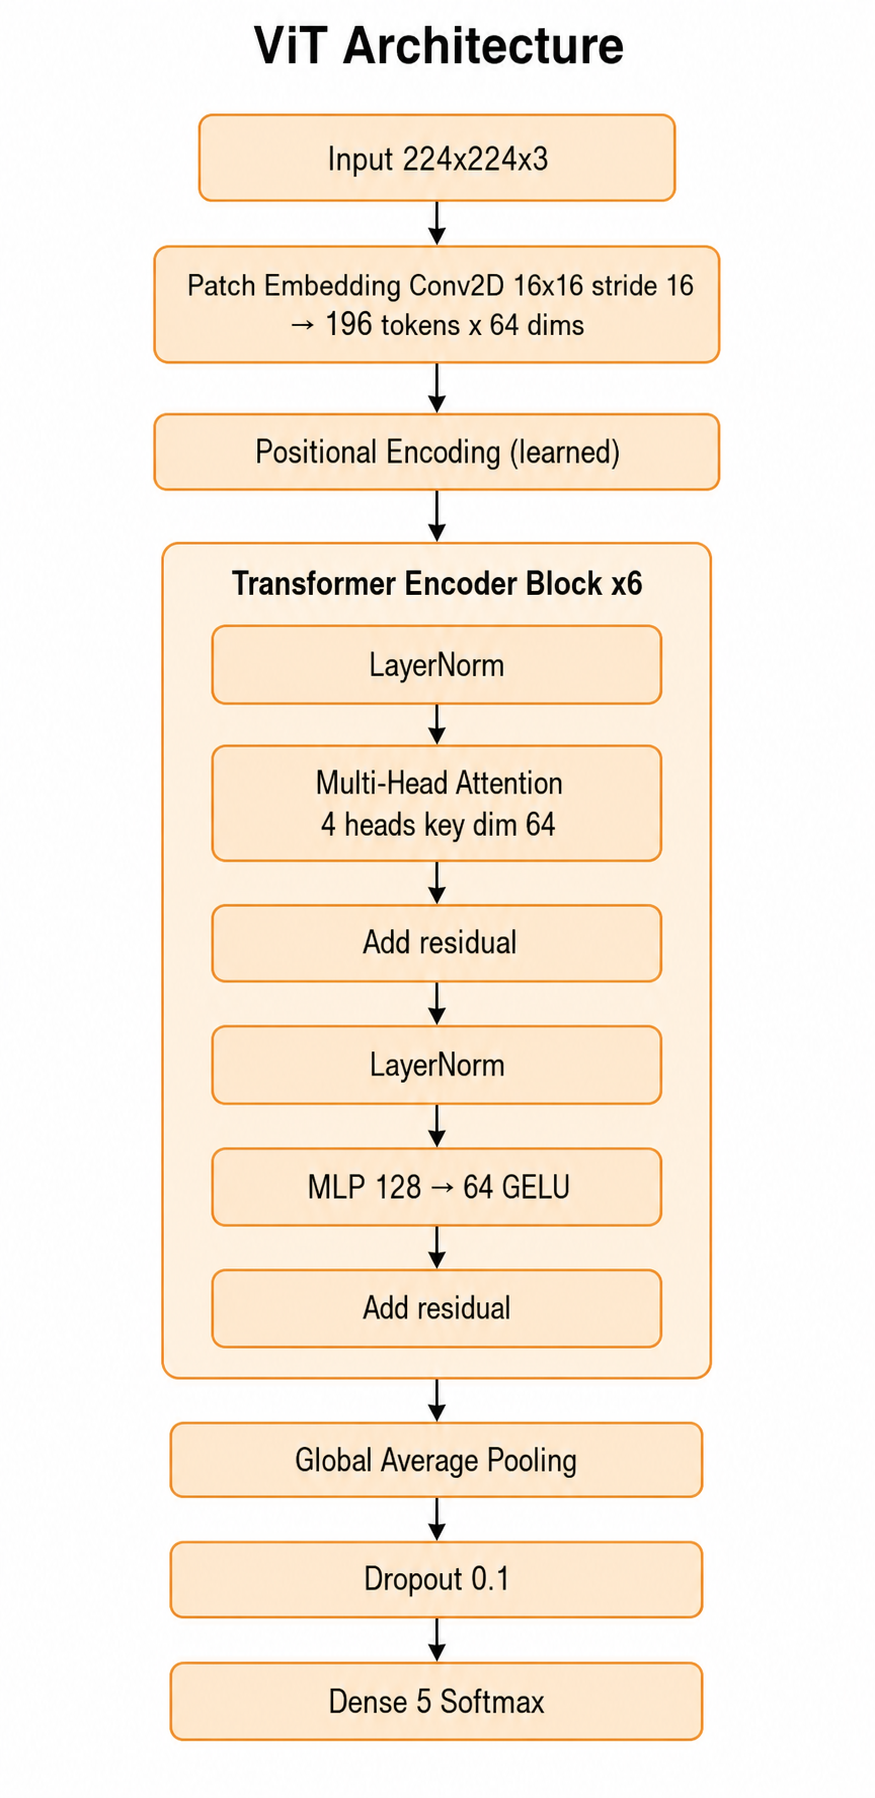
\includegraphics[width=\linewidth]{figures/vit.png}
  \captionof{figure}{ViT model overview.}
  \label{fig:vit}
  \end{minipage}
\textbf{Classification head.} After the encoder, a final \texttt{LayerNormalization} is applied to the full sequence. The 196 patch representations are then aggregated into a single vector using \texttt{GlobalAveragePooling1D}, which takes the mean across the sequence dimension. A \texttt{Dropout} layer with rate 0.1 is applied before the final \texttt{Dense} layer with 5 outputs and softmax activation, which produces the class probability distribution.

% ---------------------------------------------
\section{Training Setup}
% ---------------------------------------------

Both models are trained with the same configuration to ensure a fair comparison.
The optimiser is Adam with an initial learning rate of $10^{-3}$. Training runs
for up to 20 epochs with a batch size of 32. Three callbacks are used: early
stopping (patience 5, restores best weights), a model checkpoint (saves best
validation model), and learning rate reduction on plateau (factor 0.5, patience
3, min lr $10^{-6}$). Training wall-clock time is recorded separately for each
model.
\begin{table}[H]
\centering
\caption{Shared training hyperparameters.}
\begin{tabular}{@{}ll@{}}
\toprule
\textbf{Hyperparameter}   & \textbf{Value} \\
\midrule
Optimiser                 & Adam \\
Learning rate             & $10^{-3}$ \\
Max epochs                & 20 \\
Batch size                & 32 \\
Early stopping patience   & 5 \\
LR decay factor           & 0.5 \\
LR decay patience         & 3 \\
Minimum learning rate     & $10^{-6}$ \\
\bottomrule
\end{tabular}
\end{table}
% ---------------------------------------------
\section{Results}
% ---------------------------------------------

Both models are evaluated on the held-out test set after training. Table~\ref{tab:results}
reports the headline metrics; Figures~\ref{fig:curves_cnn}--\ref{fig:curves_vit} show the
per-epoch learning curves. The metrics
reported are test accuracy, test loss, total parameter count, and training time.

\begin{table}[H]
\centering
\caption{CNN vs.\ ViT on the test set (run \texttt{8f1ed8fb}).}
\label{tab:results}
\begin{tabular}{@{}lrrrr@{}}
\toprule
\textbf{Model} & \textbf{Params} & \textbf{Acc} & \textbf{Loss} & \textbf{Time} \\
\midrule
CNN & 11.2M & 98.71\% & 0.0427 & 351\,s \\
ViT & 0.55M & \textbf{99.49\%} & \textbf{0.0177} & 887\,s \\
\bottomrule
\end{tabular}
\end{table}

\begin{figure}[H]
\centering

\includegraphics[width=\linewidth]{learning_curves_combined.png}
\caption{Loss (left) and accuracy (right) per epoch for both models.
Solid lines: training; dashed lines: validation. Blue: CNN; orange: ViT.}
\label{fig:curves}
\end{figure}

\section{CHOOSE ONE from bellow!}

The CNN (Figure~\ref{fig:curves_cnn}) shows intermittent validation-loss spikes at
epochs 6--8 and 14 (gap up to $+0.051$), stabilized by \texttt{ReduceLROnPlateau} and
stopped early at epoch~16. The ViT (Figure~\ref{fig:curves_vit}) exhibits no such
instability: train and val loss track closely throughout, converging to its best
validation accuracy of \textbf{99.52\%} at epoch~19.

The learning curves show how validation accuracy evolves over epochs for each
model. The confusion matrices show which varieties are most often confused.
The CNN experienced intermittent validation-loss spikes at epochs 6--8 and 14
(loss gap up to $+0.051$), stabilised by \texttt{ReduceLROnPlateau}. The ViT
exhibited no such instability: val loss tracked train loss within $\pm0.02$
throughout, converging to its best validation accuracy of \textbf{99.52\%} at
epoch~19.

% ---------------------------------------------
\section{Discussion}
% ---------------------------------------------

CNNs apply small local filters that encode the prior that nearby pixels share
information --- a well-suited assumption for images. The ViT takes a different
approach: it splits the image into patches and uses self-attention to relate any
two patches regardless of spatial distance, giving more flexibility at the cost
of no built-in spatial structure.

\paragraph{Accuracy.}
Contrary to the expectation that a CNN's inductive bias would dominate on a
moderate-sized dataset, the ViT outperformed the CNN by \textbf{0.78\,pp}
(99.49\% vs.\ 98.71\%), translating to roughly 88 fewer misclassifications on
the 11\,250-image test set. Ipsala is the easiest class for both models (CNN F1
99.98\%, ViT F1 100\%), likely due to its morphologically distinct grain shape.
Visually similar long-grain types such as Basmati and Jasmine were the hardest
to separate.

\paragraph{Efficiency.}
The ViT achieves better accuracy with \textbf{20$\times$ fewer parameters}
(549K vs.\ 11.2M), demonstrating that self-attention over patch sequences can
capture discriminative features more compactly than stacked convolutions for
this task. However, it takes \textbf{2.5$\times$ longer} to train (887\,s vs.\
351\,s), reflecting the quadratic attention complexity over 196 patches.

\paragraph{Stability.}
The CNN's mid-training spikes suggest its feature hierarchy is more sensitive to
learning-rate scheduling than the ViT. A lower initial lr ($5\times10^{-4}$) or
stronger weight decay may reduce this instability.

\paragraph{Limitations.}
Both models are trained from scratch on a single dataset. Transfer learning from
ImageNet would likely improve both accuracy and training efficiency. The ViT here
is a lightweight custom baseline, not a pre-trained ViT-B/16, so direct
comparison to published ViT benchmarks is not appropriate.

% ---------------------------------------------
\section*{Conclusion}
% ---------------------------------------------

This project trained a custom CNN and a custom ViT on the same rice grain
dataset under identical conditions. Both architectures are implemented from
scratch with no pretrained weights, isolating the effect of architectural design.
Contrary to the expectation that transformers require large-scale pretraining to
match CNN performance, the ViT outperformed the CNN with 20$\times$ fewer
parameters, achieving 99.49\% test accuracy and more stable training dynamics.
The CNN remains competitive and trains 2.5$\times$ faster, making it a
reasonable choice under resource constraints.

% LEGACY BELLOW
\clearpage

\chapter{Work in progress}
\section{Training Setup}

Both models are trained with the same configuration to ensure a fair comparison. The optimizer is Adam with a learning rate of $10^{-3}$. Training runs for up to 20 epochs with a batch size of 32. Three callbacks are used for both models: early stopping with patience 5 that restores the best weights, a model checkpoint that saves the best validation model, and learning rate reduction on plateau with a factor of 0.5, patience of 3 epochs, and a minimum learning rate of $10^{-6}$. Training wall-clock time is recorded separately for each model and included in the final comparison.

\begin{table}[h]
\centering
\caption{Shared training hyperparameters}
\begin{tabular}{ll}
\toprule
\textbf{Hyperparameter} & \textbf{Value} \\
\midrule
Optimizer       & Adam \\
Learning rate   & $10^{-3}$ \\
Max epochs      & 20 \\
Batch size      & 32 \\
Early stopping patience & 5 \\
LR reduction factor     & 0.5 (patience 3, min $10^{-6}$) \\
\bottomrule
\end{tabular}
\end{table}

\section{Results}

Both models are evaluated on the held-out test set after training. The metrics reported are test accuracy, test loss, total parameter count, and training time in seconds. Per-epoch learning curves and confusion matrices are saved automatically during evaluation.

\begin{table}[h]
\centering
\caption{CNN vs. ViT comparison on the test set}
\begin{tabular}{lcccc}
\toprule
\textbf{Model} & \textbf{Parameters} & \textbf{Test Accuracy} & \textbf{Test Loss} & \textbf{Train Time (s)} \\
\midrule
CNN & & & & \\
ViT & & & & \\
\bottomrule
\end{tabular}
\end{table}

The learning curves show how validation accuracy evolves over epochs for each model. The confusion matrices show which rice varieties are most often confused with each other. Visually similar long-grain types such as Basmati and Jasmine are likely the hardest to separate for the weaker model.

\section{Discussion}

CNNs apply small local filters that slide across the image, encoding the prior that nearby pixels share information. This is a well-suited assumption for images and allows the model to learn useful texture and shape features quickly even from a modest amount of training data. The ViT takes a different approach: it splits the image into patches and uses self-attention to relate any two patches regardless of their spatial distance. This gives the model more flexibility in theory, but it also means it receives no built-in spatial structure and must learn it entirely from examples.

On a dataset of roughly 75,000 domain-specific images with no pretraining, the CNN is expected to converge faster and reach higher accuracy. Rice grain classification is largely driven by local texture, which is exactly what convolutional filters are designed to capture. The ViT's ability to model long-range relationships across the image provides less benefit for this particular task. Training time is also a relevant factor, since self-attention over 196 patches is computationally heavier per epoch than a three-block CNN at this scale.

\section{Conclusion}

This project trains a custom CNN and a custom ViT on the same rice grain dataset under identical conditions and compares their performance directly. Both architectures are implemented from scratch with no pretrained weights, which isolates the effect of architectural design on classification accuracy. Based on the structure of the task and the scale of the dataset, the CNN is expected to outperform the ViT. This is consistent with the broader finding in the literature that transformers require large-scale pretraining to match CNN performance on small to medium datasets.


\begin{thebibliography}{1}
\bibitem{rice}
M.\ Koklu et al., ``Classification of Rice Varieties with Deep Learning
Methods,'' \textit{Computers and Electronics in Agriculture}, 2021.
\end{thebibliography}

\appendix
\section*{Appendix A: Experimental Platform}

\begin{table}[H]
\centering
\caption{Experimental platform.}
\label{tab:hw}
\begin{tabular}{@{}ll@{}}
\toprule
\textbf{Component} & \textbf{Specification} \\
\midrule
\multicolumn{2}{@{}l}{\textit{Hardware}} \\[2pt]
CPU    & AMD EPYC 9354P, 32 cores / 64 threads \\
Memory & 256\,GB DDR5 \\
GPU    & NVIDIA L40S, 46\,GB GDDR6, PCIe Gen4$\times$16 \\
\midrule
\multicolumn{2}{@{}l}{\textit{Software}} \\[2pt]
OS        & Ubuntu 22.04.5 LTS, kernel 5.15.0-173 \\
CUDA      & 12.6 (V12.6.85) \\
Driver    & 580.95.05 \\
Container & Docker 29.1.3 \\
\bottomrule
\end{tabular}
\end{table}

\section*{Appendix B: Source Code}

The full source code, training scripts, Dockerfile, and results index are
publicly available at:

\begin{center}
\url{https://github.com/entroopie/ai-project-cnn-vs-vit}
\end{center}

\end{document}
